\documentclass{scrarticle}
\usepackage{graphicx} % Required for inserting images
\usepackage{amsmath}
\usepackage{amsfonts}
\usepackage{amssymb}
\usepackage{enumerate}
\usepackage{amsthm}
\newtheorem{theorem}{Theorem}[section]
\newtheorem{corollary}{Corollary}[theorem]
\newtheorem{lemma}[theorem]{Lemma}
\newtheorem{definition}{Definition}[section]
\setlength{\parindent}{0cm}
\usepackage{appendix}
\usepackage{tikz}
\usetikzlibrary{decorations.pathreplacing}
\usepackage{xurl}
\usepackage{hyperref}
\usepackage{marginnote}

%Head and Foot
\usepackage{scrlayer-scrpage}
\clearpairofpagestyles
\pagestyle{scrheadings}
\renewcommand*{\sectionmark}[1]{\markboth{#1}{}}


\ihead[]{
\includegraphics[height=1.5cm]{figures/PLUS_Logo_Farbe.png}}
\chead[]{Statistical learning theory}
\ohead[]{}
\ifoot[]{}
\cfoot[]{Dept. of Artificial Intelligence and Human Interfaces}
\ofoot*{\pagemark}

\title{Statistical learning theory}
\author{Univ.-Prof. Dr. Roland Kwitt}
\date{Summer semester 2025}

\begin{document}

\maketitle
\begin{center}
Book: Understanding Machine Learning - Shai, Sholev and Schwartz

\vspace{0cm}

Online Content: \url{http://rkwitt.org} (see at Teaching) and \url{https://github.com/rkwitt/teaching}
\end{center}


% \tableofcontents
%\newpage


\section{Introduction}

\subsection{Practice problem}
Suppose our goal is to classify a dataset of papaya's. We want to find out which papaya is tasty and which is not. Therefore, we need a function that can assert such property given a number of input features (e.g. weight, color). This function, further called hypothesis, will take a two-dimensional vector and supply us with an output indicating whether a papaya is tasty or not by the labels 0 (not tasty) and 1 (tasty).

\begin{table}[ht]
    \centering
    \begin{tabular}{c|c|c||c}
         Observation &Weight [g]  &Color [0,1]  &Tasty $\in \{0,1\}$ \\
         \hline
         Papaya 1 &100  &0.1  &yes (1) \\
         . & . & . & . \\
         . & . & . & . \\
         . & . & . & . \\
         Papaya N&500  &0.8  &no (0) \\
    \end{tabular}
    \caption{Papaya classification: Training dataset}
    \label{tab:papaya}
\end{table}

The information in the table is called the \textit{training data} $S=\{(x_1, y_1),\, \ldots \, , (x_n, y_n)\}$. In our example $x_i \in \mathbb{R}^2$ and $y_i \in \{0,1\}$. Based on that, we want to find:

\[
h: \mathbb{R} \times \mathbb{R} \to \{0,1\}
\]

\subsection{Learning}

A \textit{learner} receives $S$ and outputs a hypothesis $h$ (some algorithm, see figure \ref{fig:idea-of-learning}).

\begin{figure}
    \centering
    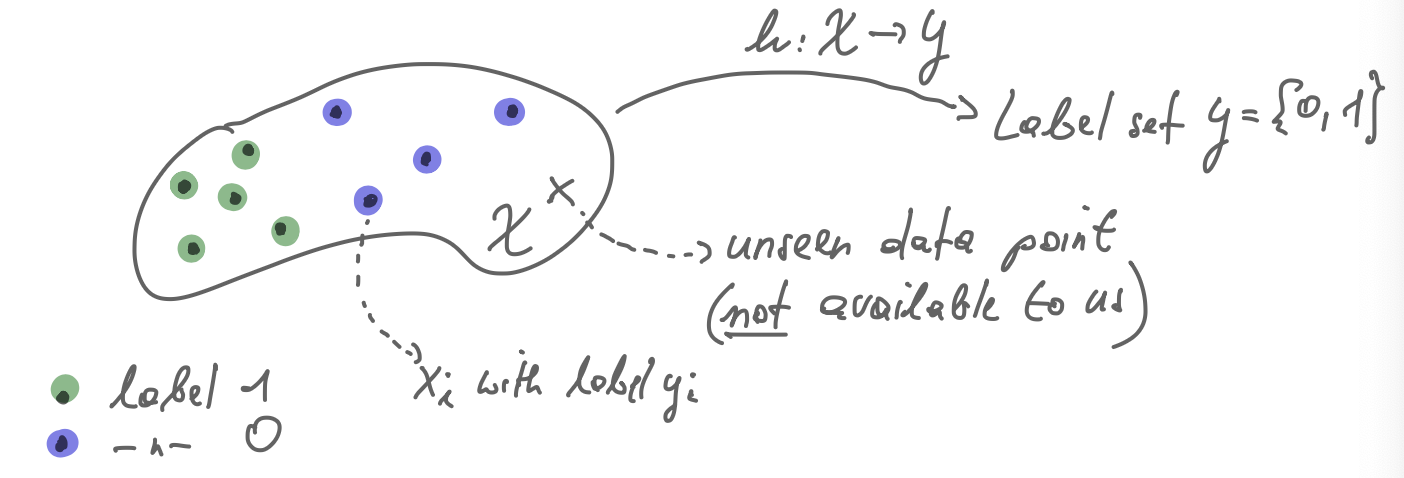
\includegraphics[width=1.0\linewidth]{figures/Learning.png}
    \caption{Idea of Learning}
    \label{fig:idea-of-learning}
\end{figure}

We will make two assumptions initially:
\begin{itemize}
    \item All the $x_i$'s are drawn \textit{independently and identically distributed} (i.i.d.) from some (unknown) distribution $\mathcal{D}$ over our domain set $X$.
    \item The $x_i$'s are labeled by some (unknown) function $f:X \to Y$ ( labeling function). This means $S=\{(x_1, f(x_1)),\, \ldots \, , (x_n, f(x_n)\} $
\end{itemize}

We care about, whether the hypothesis makes an incorrect prediction (with respect to $f$). These are all the points $x$ in our domain $X$, where the hypothesis $h$ differs from the labeling function $f$. In our example $X=\mathbb{R}^2$ so let's say $A \in \mathcal{P}(\mathbb{R}^2)$.

$A=\{x \in X | h(x) \neq f(x)\}$ (misclassifications) 

\begin{enumerate}
    \item Domain set $X$, we call $x \in X$ an instance
    \item Label set $Y$, e.g. $Y=\{0,1\}$
    \item Training set $S=\{(x_1,y_1),\, \ldots \, , (x_m, y_m)\}$ with $(x_i, y_i) \in X \times Y := Z$
    \item A learner receives $S$ and outputs $h:X \to Y$ (e.g. a hypothesis)
\end{enumerate}

\subsection{Measure problem}

Find $\mu:\mathcal{P}(\mathbb{R}^n) \to [0,\infty]$ with the following properties: 
\begin{enumerate}[I.]
    \item $A_i \in \mathcal{P}(\mathbb{R}^2),\, i \in \mathbb{N}$ pairwise disjoint $\mu \big (\bigcup_{i=1}^\infty \Big ) = \sum_{i=1}^\infty \mu(A_i)$
    \item If $A,B \in \mathcal{P}(\mathbb{R}^2)$ is congruent: $\mu(A) = \mu(B)$
    \item $\mu ({[0,1]}^n)=1$
\end{enumerate}

This problem is not solvable for all $n \in \mathbb{N}$ (unless we'd accept $\mu \equiv 0$). We will constrain $\mathcal{A}$ to be an element of a $\sigma$-Algebra over $X$. Later, we will be talking about quantities of the form:

\begin{equation}
    \underset{x \sim \mathcal{D}}{\mathbb{P}}\big [h(x) \neq f(x) \big] = \mathcal{D} \big (\{x \in X: h(x) \neq f(x) \} \big ) \marginnote{\small{Generali\-zation error}}
\end{equation}

\section{Statistical learning theory}
More formally, the data that is available to us comes in the form: 
\begin{equation}
    S=\big ((x_1, y_1),\, \ldots \, , (x_n, y_n) \big)
\end{equation}

The \textit{training set} is based on the \textit{domain set} $X$, where we call $x \in X $ an instance and $Y$, the label set (e.g. $Y=\{0,1\}$. Thus, a learner receives $S$ and outputs a \textit{hypothesis} $h:X \to Y$ (by some algorithm). In the papaya example, the domain is $x_i \in \mathbb{R}^2$ and the label set $y_i \in \{0,1\}$.

We'll make two assumptions initially:
\begin{enumerate}
    \item All the $x_i$'s are drawn independently and identically distributed (iid) from some (unknown) distribution $\mathcal{D}$ over the domain $X$.
    \item The $x_i$'s are labeled by some (unknown) function $f: X \to Y$, called the labeling function. This means $S=\big ((x_1, y_1=f(x_1)),\, \ldots \, , (x_n, y_n = f(x_n)) \big )$
\end{enumerate}

We care about all the points $x$ in our domain $X$, where the hypothesis $h(x)$ differs from the true labeling function $f(x)$.
\begin{equation*}
    A = \{x \in X: h(x) \neq f(x)\}
\end{equation*}

\section{No free lunch}
There is no generally perfect method. What we really do, when restricting the search space (e.g. for ERM) to a class $\mathcal{H}$ is to hope that one $h \in \mathcal{H}$ has \textit{low error}. This is a form of \textit{prior knowledge}. The question now is, if this is really necessary?

What if there is some form of \textit{universal learner}? That is, a learner that succeeds on any given task (defined by distribution $\mathcal{D} \text{ over } X \times Y$). By \textit{succeed} we mean finding a $h: X \to Y$ with low risk ($L_D(h)$). 

We will show, for the task of binary classification, that no such learner exists. In particular, we show that there exists a distribution, such that upon receiving $m$ samples from that distribution, the learner outputs a hypothesis with high risk, respectively generalization error, while another learner exists with small risk. So every learner has tasks on which it fails, while others succeed in learning the same task. 

\begin{theorem}[No free lunch]
Let $A$ be any learning algorithm for binary classification with respect to the $0-1$ loss over a domain $X$. Further, let $m < \frac{|X|}{2}$. Then, there exists a distribution $\mathcal{D} \text{ over } X \times \{0,1\}$ such that: 
\begin{enumerate}
    \item $\exists f: X \to \{0,1\} \text{ with } L_D(f) = 0$ 
    \item $\mathcal{D}^m(\{S:L_D(A(S)) \geq \frac{1}{8})\geq \frac{1}{7}$ \hspace{1cm} ($\text{with } |S|=m$)
\end{enumerate}
\end{theorem}

\begin{proof}
Let $C \subset X$ of size $2m$. The number of possible labellings of $C$ is $T=2^{2m}$. We denote the functions that realize all these labellings by $f_1, \ldots ,f_T$. For each $f_i$, we define:

\begin{equation*}
    \mathcal{D}_i (\{(x,y)\}) = \begin{cases} \frac{1}{|C|} & \text{if } y=f_i(x) \\0 &  \text{else}\end{cases}
\end{equation*}


We see that $L_D(f_i) = 0$ (by construction).

We are going to that show, that $\exists\,\mathcal{D} \text{ over } X \times \{0,1\}$ and a function $f: X \to \{0,1\}$ such that $L_D(f)=0$, but the expectation: 

\begin{equation*}
\underset{S\sim D}{\mathbb{E}} \Big [ L_D(A(S) \Big ] \geq const.
\end{equation*}

To that end, we aim to prove: 
\begin{equation*}
    \max_{i \in \{1,2,3,\ldots\}} \Big ( \underset{S\sim D}{\mathbb{E}} \Big [ L_D(A(S) \Big ] \geq const. \Big )
\end{equation*}

\textbf{Step 1} We know that there are $(2m)^m$ possible training sets of size $m$. 

Ex. $C=\{c_1, c_2\}$, $m=1$

We have $\{c1\}$ or $\{c1\}$

\end{proof}


\section{Lecture 20.05.25}

\textbf{Question.} Is there a universal learner? By a universal learner we mean a learner without any prior knowledge of the learning task (given by $\mathcal{D}$), but can be challenged by any task and still returns $A(S)$ with low generalization error $L_D(A(S))$ 

This question is answered by the following theorem:

\begin{theorem}[No free lunch]
\label{theo:nofreelunch}
Let $A$ be a learning algorithm for the task of binary classification with respect to the 0-1 loss, over domain $X$. Also, let $m \in \mathbb{N}$ be any number smaller than $\tfrac{|X|}{2}$ (representing the size of S). Then, there exists a distribution $\mathcal{D}$ over $X \times \{0,1\}$, such that: 

\textbf{see enumeration above, at no free lunch}


This means that whatever you see on the training set, you can see anything on the test set. Without any assumption about the learning task, there is no learning. 

\medskip

\textbf{Interpretation.} 1 means that the task can be learned successfully (perfectly) by another learner (e.g. $\mathcal{H}=\{f\}$) and 2 means that $A$ fails on that task.

\end{theorem}

\begin{corollary}
Let $X$ be infinitely large and $\mathcal{H}$ be the class of all functions from $X \to \{0,1\}$, then $\mathcal{H}$ is not PAC learnable.
\end{corollary}

\subsection{Vapnik-Chervonkis Dimension (VC-Dimension)}

\textbf{Definition.} Let $\mathcal{H}$ be a class of functions from $X \to \{0,1\}$ and let $C \subset X, C=\{c_1, \ldots, c_n\}$. We define: 

\begin{equation*}
    H_c = \Big\{(h(c_1), h(c_2), \ldots , h(c_n)): h \in \mathcal{H} \Big \}
\end{equation*}
as restriction of H to the sett $C$

Example: $C=\{c_1\}, c_1 \in \mathbb{R}$ and let $H^{threashold}$ be the cals of thresholds an the real line. 

\begin{figure}[ht]
    \centering
    \begin{tikzpicture}
        \draw[<-] (-5,0) -- (0,0);
        \draw[->] (0,0) -- (5,0)  node[anchor=west] {$\mathbb{R}$};
        \draw[red, dashed] (0,0.5) -- (0,-0.5);
        \filldraw [gray] (-3,0) circle (2pt) node[anchor=south] {Label as 1};
        \filldraw [gray] (3,0) circle (2pt) node[anchor=south] {Label as 0};
    \end{tikzpicture}
    \caption{Grafik 1}
    \label{fig:R-space}
\end{figure}


\begin{equation*}
H_C^{thr} \{(1), (0)\} \rightarrow { |H_C^{thr}|} =2
\end{equation*}

Let's take $C=\{c_1, c_2\}$, $c_1 \leq c_2$

\vspace{1cm}

\begin{figure}[ht]
    \centering
    \begin{tikzpicture}
        \draw[<->] (-5,0) -- (5,0) node[anchor=west] {$\mathbb{R}$};
        \draw[red, dashed] (-2,0.5) -- (-2,-0.5); 
        \draw[red, dashed] (2,0.5) -- (2,-0.5); 
        \draw[red, decorate, decoration={brace, amplitude=10pt}, thick] 
        (-2,0.5) -- (2,0.5) 
        node[midway, yshift=16pt] {$\varepsilon$-mass};
        \filldraw [gray] (-3,0) circle (2pt);
        \filldraw [gray] (3,0) circle (2pt);
    \end{tikzpicture}
    \caption{Grafik 2}
    \label{fig:R-space2}
\end{figure}



\vspace{1cm}

We get $H_C^{thr}$

\vspace{1cm}

\textbf{GRAFIK 3}

\vspace{1cm}

But we would have $2^2 = 4$ possible labellings of $\{c_1, c_2\} = C$

\vspace{0.5cm}

\textbf{Def.} (Shattering) H shatters a finite set C of size m of $|H_C|=2^m$

\vspace{0.5cm}

\textbf{Claim.} The class $H^{thr}$ on $X=\mathbb{R}$ is \textit{PAC learnable} with 

\begin{equation*}
    m_{H^{thr}} (\varepsilon, d) \leq \lceil \log (\frac{2}{\delta}) \cdot \frac{1}{\varepsilon} \rceil
\end{equation*}

\begin{equation*}
    H^{thr}_C = \{(1,1), (0,0), (1,0)\} \rightarrow |H_C| = 3
\end{equation*}

\textcolor{red}{Here is something missing}

\begin{figure}[ht]
    \centering
    \begin{tikzpicture}
        \draw[<->] (-5.5,0) -- (-2.5,0);
        \filldraw [gray] (-4.5,0) circle (2pt);
        \filldraw [gray] (-3.5,0) circle (2pt);
        \draw[red, dashed] (-3,0.5) -- (-3,-0.5) node[anchor=west] {0} node[anchor=east] {1}; 
        
        \draw[<->] (-1.5,0) -- (1.5,0);
        \filldraw [gray] (-0.5,0) circle (2pt);
        \filldraw [gray] (0.5,0) circle (2pt);
        \draw[red, dashed] (-1,0.5) -- (-1,-0.5) node[anchor=west] {0} node[anchor=east] {1};
        
        \draw[<->] (2.5,0) -- (5.5,0) node[anchor=west] {$\mathbb{R}$};
        \filldraw [gray] (4.5,0) circle (2pt);
        \filldraw [gray] (3.5,0) circle (2pt);
        \draw[red, dashed] (4,0.5) -- (4,-0.5) node[anchor=west] {0} node[anchor=east] {1}; 

        
    \end{tikzpicture}
    \caption{Threshold}
    \label{fig:threshold}
\end{figure}


We assume realization, e.g., $\exists h^x \in H^{thr}$ such that $L_{D,f}(h^x)=0$.

\vspace{1cm}

\begin{figure}[ht]
    \centering
    \begin{tikzpicture}
        \draw[<->] (-5,0) -- (5,0) node[anchor=west] {$\mathbb{R}$};
        \draw[red, dashed] (-2,0.5) -- (-2,-0.5); 
        \draw[red, dashed] (2,0.5) -- (2,-0.5); 
        \draw[red, decorate, decoration={brace, amplitude=10pt}, thick] 
        (-2,0.5) -- (2,0.5) 
        node[midway, yshift=16pt] {error margin};
        \filldraw [gray] (-3,0) circle (2pt);
        \filldraw [gray] (3,0) circle (2pt);
    \end{tikzpicture}
    \caption{Threshold}
    \label{fig:threshold2}
\end{figure}

\vspace{1cm}

We let an $a_0 \in \mathbb{R}$ be such that: 

\begin{equation*}
    \mathbb{D}\Big ( \{x \in \mathbb{R}\: x \in (a_0, a^*) \} \Big )=\varepsilon
\end{equation*}

and let $a_1 \in \mathbb{R}$ be such that:

\begin{equation*}
    \mathbb{D}\Big ( \{x \in \mathbb{R}\: x \in (a_*, a^1) \} \Big )=\varepsilon
\end{equation*}

\textbf{Special cases.} 
\begin{equation*}
\mathbb{D}\Big ( \{x \in \mathbb{R}: x \in (a_0, a^*) \} \Big ) < \varepsilon, \text{a set } a_0 = -\infty
\end{equation*}

\begin{equation*}
\mathbb{D}\Big ( \{x \in \mathbb{R}: x \in (a^*, a_1) \} \Big ) < \varepsilon, \text{a set } a_1 = +\infty.
\end{equation*}

\begin{figure}[ht]
    \centering
    \begin{tikzpicture}
        \draw[<->] (-5,0) -- (5,0) node[anchor=west] {$\mathbb{R}$};

        \filldraw [gray] (-3,0) circle (2pt) node[anchor=north]{$a_0$};
        \filldraw [gray] (0,0) circle (2pt) node[anchor=north]{$a^*$};
        \filldraw [gray] (4,0) circle (2pt)node[anchor=north]{$a_1$};

        
        \draw[decorate, decoration={brace, amplitude=10pt}, thick] 
        (-3,0.5) -- (0,0.5) 
        node[midway, yshift=16pt] {$\varepsilon$-mass 1};

        
        \draw[decorate, decoration={brace, amplitude=10pt}, thick] 
        (0,0.5) -- (4,0.5) 
        node[midway, yshift=16pt] {$\varepsilon$-mass 2};
    \end{tikzpicture}
    \caption{$\varepsilon$-mass}
    \label{fig:epsilon-mass}
\end{figure}

Next, we are going to define an ERM algorithm (needed) for PAC)

\begin{figure}[ht]
    \centering
    \begin{tikzpicture}
        \draw[<->] (-5,0) -- (5,0) node[anchor=west] {$\mathbb{R}$};
        \draw[dashed, ->] (-2,1) node[anchor=west]{$b_0$} -- (-2,0.2) ; 
        \draw[dashed, ->] (2,1) node[anchor=west]{$b_1$} -- (2,0.2); 

        \filldraw [green] (-2,0) circle (2pt);
        \filldraw [green] (-2.7,0) circle (2pt);
        \filldraw [green] (-3.5,0) circle (2pt);
        \filldraw [red] (2,0) circle (2pt);
        \filldraw [red] (3.1,0) circle (2pt);
        \filldraw [red] (3.8,0) circle (2pt);
    \end{tikzpicture}
    \caption{ERM-Algorithm}
    \label{fig:erm-algo}
\end{figure}

Pick $b_0 \in \mathbb{R}$ and $b_1 \in \mathbb{R}$ from $S=((x_1, y_1), \ldots , (x_n, y_n))$ as:

\begin{equation*}
    b_0 = \max \{x:(x,1) \in S\} 
\end{equation*}
\begin{equation*}
    b_1 = \min \{x:(x,0) \in S\} 
\end{equation*}

Then, pick any threshold within $(b_0, b_1)$ and call the corresponding hypothesis $h_S$. We see, $h_s$ always has $0$ empirical error on $S$. 

By our construction of $a_0$ and $a_1$, the claim is that for $h_S$ (ERM hypothesis, threshold $a_s$) to have a generalization error $L_{D, f} (h_S) \leq \varepsilon$, it suffices that: 

\begin{enumerate}[(a)]
    \item $b_1 \leq a_1$ 
    \item[] AND
    \item $b_0 \geq a_0$
\end{enumerate}

\begin{figure}[ht]
    \centering
    \begin{tikzpicture}
        \filldraw[yellow!30] (0,0.2) rectangle (5,0);
        \filldraw[green!30] (0,0.2) rectangle (-5,0);
        \draw[<->] (-5,0) -- (5,0) node[anchor=west] {$\mathbb{R}$};

        \filldraw [gray] (-3,0) circle (2pt) node[anchor=north]{$a_0$};
        \filldraw [gray] (0,0) circle (2pt) node[anchor=north]{$a^*$};
        \filldraw [gray] (4,0) circle (2pt)node[anchor=north]{$a_1$};

        
        \draw[decorate, decoration={brace, amplitude=10pt}, thick] 
        (-3,0.5) -- (0,0.5) 
        node[midway, yshift=16pt] {$\varepsilon$-mass 1};

        
        \draw[decorate, decoration={brace, amplitude=10pt}, thick] 
        (0,0.5) -- (4,0.5)        node[midway, yshift=16pt] {$\varepsilon$-mass 2};
    \end{tikzpicture}
    \caption{Grafik 7}
    \label{fig:graphic7}
\end{figure}

\section{Lecture 27.05.2025}

If we it write down formally, we have the following: 


\begin{align}
        \mathbb{P} \Big [ L_{D,S} (h)  > \varepsilon \Big ] &\leq \mathbb{P}\ \Big [(b_0 < a_0) \wedge (b_1 > a_1) \Big ] \marginnote{Union Bound} \\
        &\leq \mathbb{P}\ \Big [b_0 < a_0\Big ]+ \mathbb{P}\Big [ b_1 > a_1) \Big ] 
\end{align}

The upper bound $\mathbb{P}[L_{D,f}(h) > \varepsilon]$, we have to check when $b_0 < a_0$ (or $b_1 > a_1$). Answer: when there is no data-point in S that is labeled 1, such that $x \in (a_0, a^*)$.

We know that $D(\{x \in \mathbb{R}: x \in (a_0, a^*)\})=\varepsilon$ (by construction of $a_0$), hence, \textit{not seeing} a data-point in $(a_0, a^*)$ has probability of $1-\varepsilon$. Consequently, \textit{not seeing} a data-point in $m$ i.i.d. samples (inside $(a_0, a^*)$) has probability $(1-\varepsilon)^m$.
 
Overall we have:
\begin{equation*}
    \mathbb{P}[L_{D,S}(h) > \varepsilon] \leq 2 \cdot (1-\varepsilon)^m \leq 2\exp(-\varepsilon m)
\end{equation*}

BOXED(
\begin{equation*}
    m > \frac{1}{\varepsilon}  \log(2 / \delta)
\end{equation*}
Sample complexity. 
)


Thresholds are PAC-learnable 

We have seen that \textit{finiteness} of H is \textbf{sufficient}, but not \textbf{necessary} for PAC learnability. 


\begin{definition}[VC-Dimension]
    The VC-Dimension of H (e.g. a class of functions for $X \to \{0,1\}$ written as $VC(X)$, is the maximal size of a set $C \subset X$, that is shattered by H.
\end{definition}

\begin{theorem}
    Let H be a class of functions from $X \to \{0,1\}$. If H has infinite VC-Dimension, then H is not PAC-learnable. This follows immediately from Theorem \ref{theo:nofreelunch} (\textit{No Free Lunch}).
\end{theorem}

\begin{definition}[Growth-function]
    Let H be a class of functions from $X \to \{0,1\}$. The \textit{growth function} $\tau_H: \mathbb{N}_0 \to \mathbb{N}_0$ is defined as: 

    \begin{equation}
        \tau_H(m)= \max |H_c| : |C|=m,  C \subset X
    \end{equation}
\end{definition}

\begin{lemma}[Sauer's lemma (Sauer, Shelak, Perez)]
    Let H be a class of functions from $X \to \{0,1\}$ with $VC(H) = d < \infty$. Then, 
    \begin{equation}
    \tau_H(m) = 2^m \text{ , if } m\leq d \text{, but} 
    \end{equation}
    \begin{equation}
    \tau_H(m) = \big (\frac{e \cdot m}{d}\big )^d\text{, if } m>d \quad\text{(VC-Dimension)} 
    \end{equation}
\end{lemma}

Lets take any set C of size m and $|H|<\infty$ is finite, then we know $|H_C| \leq |H|$. So, if $|H| <2^m $, then H can obviously not shatter C of size m. This implies 

\begin{equation}
    VC(H) \leq \log_2(|H|)
\end{equation}

\begin{theorem}
    Let H be a class of functions from $X \to \{0,1\}$ and $l: H \times X \times Y \to [0,c]$, $c>0$, a loss function. For any distribution D over $X \times Y$ and $\delta \in (0,1)$, we have with probability of at least $1-\delta$ (over the choice of $S \sim D^m$): 

    \begin{equation}
        \forall h \in H: |L_D(h)-L_S(h)| \leq \sqrt{\frac{8 \cdot \log \big (\tau_H(2m) \cdot  \frac{4}{\delta} \big )}{m}}
    \end{equation}
\end{theorem}

This means that, as the sample set gets larger, the generalization error and the empirical error come closer together. 














\appendix

\section{Preliminaries}

\subsection{Sigma-Algebra}
Let $S$ be a non-empty set. A family of sets $\mathcal{F} \subset \mathcal{P}(S)$ is called a $\sigma$-Algebra on $S$, if the following conditions hold: 

\begin{enumerate}[I.]
    \item  $S \in \mathcal{F}$
    \item From $A \in \mathcal{F}$, it follows that $A^C=S \setminus A \in \mathcal{F}$
    \item $A_i \in \mathcal{F},\,i\in \mathbb{N}$, it follows that $\bigcup_{i=1}^\infty A_i \in \mathcal{F}$
\end{enumerate}

\textbf{Remark.} Any subset $\mathcal{F} \subset \mathcal{P}(S)$ is called a family of of sets. Smallest $\sigma$-Algebra over $S: \{\emptyset, S\}$
$\sigma$-Algebra generated by $A: \text{if}\, A \subset S$, than $\sigma (A) = \{ \emptyset, A, A^C, S \}$ is the $\sigma$-Algebra generated by $A$.


\subsection{Generators}
Let $\varepsilon \subset \mathcal{P}(S)$ be a family of sets. Further, let $\sum$ be the set of all $\sigma$-Algebra over S that contain $\varepsilon$. Then, 
\begin{equation}
    \sigma(\varepsilon) = \underset{\mathcal{F \in \sum}}{\bigcap} \mathcal{F}
\end{equation}

is called the $\sigma$-Algebra generated by $\varepsilon$.
\vspace{0.3cm}

\textbf{Example.} 

\begin{equation*}
    \varepsilon = \big \{ \{1\} \big \} \text{ and } S=\{1,2,3\}
\end{equation*}
\begin{equation*}
    \sigma(\varepsilon) = \sigma \Big (\big \{ \{1\} \big \} \Big ) = \big \{\emptyset, \{1\}, \{2,3\}, \{1,2,3\} \big \}
\end{equation*}

\begin{equation*}
    \varepsilon = \big \{ \{a\}, \{b\} \big \} \text{ and } S=\{a,b,c,d\}
\end{equation*}

\begin{equation*}
    \sigma (\varepsilon) = \big \{ \emptyset, S, \{a\}, \{b\}, \{a, b\}, \{b, c, d\}, \{a, c, d\}, \{c, d\} \big \} 
\end{equation*}

\subsection{Topological space}
A topological space is a tuple $(X, \tau)$, where $X$ is a set and $\tau$ a collection of subsets of $X$, such that:
\begin{enumerate}[I.]
    \item $\emptyset, X \in \tau$
    \item closed under union, e.g. $\big \{ u_i \big \}_{i \in I} \subseteq \tau \implies \underset{i \in I}{\bigcup} u_i\in \tau$
    \item closed under finite intersection $\big \{ u_i \big \}_{i}^n \subseteq \tau \implies \underset{i=1}{\overset{n}{\bigcap}} u_i \in \tau$ (Elements of $\tau$ are called open sets)
\end{enumerate}

\textbf{Example.} If $X = \{1,2,3,4\}$, then $\tau =  \big \{\emptyset, \{1,2,3,4\}, \{2\}, \{1,2\}, \{2,3\}, \{1,2,3\} \big \}$

\subsection{Borel-Sigma-Algebra}
Let $S$ be a topological space and $\tau$ the system of open subsets of S. Then $\mathcal{B}(S) = \sigma(\tau)$ is called the Borel-$\sigma$-Algebra over $S$. Of special interest to us is the Borel-$\sigma$-Algebra over $\mathbb{R}^n$. Elements $A \in \mathcal{B}(S)$ are called Borel sets. For $S=\mathbb{R}^n$, we write $\mathcal{B}^n=\mathcal{B}(\mathbb{R}^n)$. Each of the following families of sets is a generator for $\mathcal{B}^n$:

\begin{itemize}
    \item $\{U \subset \mathbb{R}^n:U \, \text{open}\}$
    \item $\{A \subset \mathbb{R}^n:A \, \text{closed} \}$
    \item $\{\,]a,b]:a,b \in \mathbb{R}^n, a \leq b \}$ (coordinate wise)
    \item $\{]-\infty, c]:c \in \mathbb{R}^n\}$ respectively $]-\infty, c_1] \times \, ]-\infty, c_2] \times \ldots \times \, ]-\infty, c_n] \subset \mathbb{R}^n$ $c=(c_1, \, \ldots \, , c_n) \in \mathbb{R}^n$
\end{itemize}

\subsection{Measureable space}
If $\mathcal{F}$ is a $\sigma$-Algebra over $S$, we call $(S, \mathcal{F})$ a measureable space.

\vspace{0.3cm}

\textbf{Example.} $\big (\mathbb{R}^n, \mathcal{B}(\mathbb{R}^n) \big )$

\subsection{Measureable map}
Given $(S_1, \mathcal{F}_1)$ and $(S_2, \mathcal{F}_2)$ measurable spaces, we call $f: S_1 \to S_2$, $(\mathcal{F}_1, \mathcal{F}_2)$-measurable if $\forall E \in \mathcal{F}_2: f^{-1}(E) \in \mathcal{F}_1$. Given $(S_1, \mathcal{F}_1)$ and $(S_2, \mathcal{F}_2)$ with $\mathcal{F}_2 = \sigma(\varepsilon)$, where $\varepsilon$ is the generator, the mapping $f:S_1 \to S_2$ is measureable, if $\forall E \in \varepsilon:f^{-1} \in \mathcal{F}_1$ (e.g. we just need to check generators).

\vspace{0.3cm}

\textbf{Remark.} If $f$ is continious, then $f$ is measurable.

\vspace{0.3cm}

\textbf{Example.} $I_A: S \to \mathbb{R}$


\subsection{Measure}

Let $(S, \mathcal{F})$ be a measureable space. A function $\mu: \mathcal{F} \to \mathbb{R} \cup \{+ \infty, -\infty\} = \bar{\mathbb{R}}$ is called \textit{measure}, if:

\begin{enumerate}[I.]
    \item $\mu(\emptyset) = 0$
    \item $\mu(A) \geq 0$, for all $A \in \mathcal{F}$
    \item For every sequence $(A_n)_{n \in \mathbb{N}}$ of disjoint sets from $\mathcal{F}$:
        
        $\mu \; \big (\bigcup_{i=1}^\infty A_i \big ) = \sum_{i=1}^\infty \mu \, (A_i) $
        
        This property is called $\sigma$-Additivity.
\end{enumerate}

\vspace{0.3cm}

\textbf{Remark.} Similar to $\mathcal{B}(\mathbb{R}^n)$, we define $\mathcal{B}(\bar{\mathbb{R}}_n)$.

\vspace{0.3cm}

\textbf{Example} (Counting measure). $\mu: \mathcal{F} \to \bar{\mathbb{R}}$

\begin{equation*}
    A \mapsto \begin{cases} |A|, \text{if } A \text{ finite} \\ \infty, \text{else} \end{cases}
\end{equation*}

\subsection{Measure space}

If $(S,\mathcal{F})$ is a measureable space and $\mu: \mathcal{F}\to \bar{\mathbb{R}}$ a measure, we call $(S, \mathcal{F}, \mu)$ a \textit{measure space}.

Some elementary properties of measure: Let $(S, \mathcal{F}, \mu)$ be a measure space. Also, let $A, B, A_n \in \mathcal{F}, n \in \mathbb{N}$. Then, it holfs that: 

\begin{enumerate}[I.]
    \item if $A$ and $B$ are disjoint, then $\mu\,(A \cup B) = \mu\,(A) + \mu\,(B)$
    \item if $A \subset B$ and $\mu\,(A) < \infty$, then $\mu \,(B \setminus A) = \mu\,(B) - \mu\,(A)$
    \item if $A \subset B$, then $\mu\,(A) \leq \mu\, (B)$
    \item Sub-$\sigma$-Additivity: $\mu\,\big( \bigcup_{n=1}^\infty A_n\big) \leq \sum_{n=1}^\infty \mu\,(A_n)$
\end{enumerate}

\subsection{Probability space}

Given that $(S,\mathcal{F}, \mathcal{D})$ is a measure space and $\mathcal{D}(S)=1$, then we call $\mathcal{D}$ a probability measure and $(S, \mathcal{F}, \mathcal{D})$ a probability space. 

Some explanations: 

$S \ldots$the set of \textit{outcomes} of a random experiment.

$\mathcal{F}\ldots$the set of \textit{events} to which we want to assign a probability.

$\mathcal{D}\ldots$ Assigns to each event $A \in \mathcal{F}$ a probability $\mathcal{D}(A)$, $\mathcal{D}: \mathcal{F} \to [0,1]$.

\textbf{Remark.} A possibility to contruct, based on a measure and a measureable function, a new measure.

$(S_1, \mathcal{F_1, \mu})$ measure space

$(S_2, F_2)$ measureable space

$f: S_1 \to S_2$ measureable map

Here, $\mu_f$ is called the \textit{push-forward} measure of $\mu$ under $f$.

\subsection{Random variable}

If $S_1, F_1, \mathcal{D}$ is a probability space and $(S_2, \mathcal{F}_2)$ a measureable space, them a $(\mathcal{F}_1 - \mathcal{F}_2)$ measureable function. $X: S_1 \to S_2$ is called a random variable. If $S_2 = \mathbb{R}^n$, we say $X$ is an n-dimendional real random variable. 

Importantly, the push-forward measure $\mathbb{P}_X$ on $S_2$ is also a probability mesasure. Why? 

\begin{equation}
    \mathbb{P}_X(S_2) = \mathcal{D}(X^{-1}\, (S_2)) = \mathcal{D}(S_1) = 1
\end{equation}

We call the push forward probability measure $\mathbb{P}_X$, the distribution of $X$.

Some conventions:

$\{x \in A\} = \{w \in S: X(w) \in A\}$

$\{X = c\} = \{w \in S: X(w) = c\}$

$\mathbb{P}_X(A) = \mathcal{D}(\{w \in S: X(w) \in A\})$

$\mathbb{P}_X(\{c\}) = \mathcal{D}(\{w \in S: X(w) = c\})$


\subsubsection{Expectation}

We will be taking a lot about expectation values. Hence, it makes sense to take a short detour of how expectation is defined. 

We are going to start off with a motivation for something called the \textit{Lebesgue integral}. 

Riemann-Integral (Idea): $f: \mathbb{R} \to \mathbb{R}$. The Riemann-Integral has some limitations, though. It can't be extended to higher dimensions and it relies on continuity (e.g. $f: \mathbb{R}^2 \to \mathbb{R}$

\begin{figure}
    \centering
    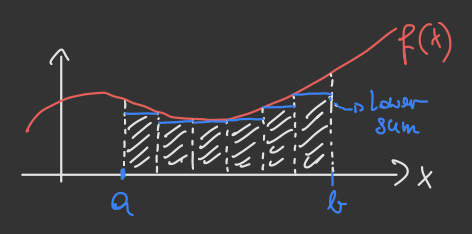
\includegraphics[width=0.5\linewidth]{figures/RiemannIntegral.png}
    \caption{Riemann Integral}
    \label{fig:riemann}
\end{figure}

\begin{figure}
    \centering
    
\includegraphics[width=0.5\linewidth]{RiemannLimitations.png}
    \caption{Riemann Limitations}
    \label{fig:riemann-lim}
\end{figure}

These issues are really a problem for us, as we will be dealing with probability spaces, $(S, \mathcal{F}, \mathcal{D})$ and random variables, e.g. $X: S \to \mathbb{R}$, so measureable functions. 

\textbf{Lebesgue Integration (Idea).} Before we partitioned the domain of f, $f: \mathbb{R} \to \mathbb{R}$. Now we partition the first part. 


This is no longer $\mathbb{R}$, but some set, just shown as a line for visualization purposes. In this manner, we can also define upper an lower sums. But, we need a way to measure $A_i$. If we can do that, we can write, e.g. $c_i \cdot \mu(A_i)$, where $\mu$ is the measure.
\begin{figure}
    \centering
    
\includegraphics[width=0.5\linewidth]{lebesgue.png}
    \caption{Lebesgue integral}
    \label{fig:lebesgue}
\end{figure}

Basically, this allows us to write: 

\begin{equation*}
    \sum_i c_i \cdot \mu(A_i) \longrightarrow \int_S f d\mu
\end{equation*}

Integration of $f$ with regard to the measure ($\mu$).

In our case, we have $(S,\mathcal{F}, \mathcal{D})$, hence we already have a measure (in particular a probability measure).

Now with a little bit more detail: Legesgue integration for simple functions, say we have a measure space $(S, \mathcal{F}, \mathcal{D})$ with $\mu:\mathcal{F} \to [0,\infty]$

Example of a simple function: 

\begin{equation*}
    \mathbb{1}_A: S \to \mathbb{R}, A \in F
\end{equation*}

Any reasonable notion of integration of $\mathbb{1}_A$ should return $\mu(A)$, i.e., 

\begin{equation*}
    I(\mathbb{1}_A) = \mu(A) \qquad I\ldots\text{Integral}
\end{equation*}

\begin{figure}
    \centering
    
\includegraphics[width=0.5\linewidth]{SimpleFunction.png}
    \caption{Simple function 1}
    \label{fig:simplefunction1}
\end{figure}

What is a \textit{simple function} now: 

\begin{equation*}
    f(x) = \sum^n_{i=1}c \cdot \mathbb{1}_{A_i}(x)
\end{equation*}
$A_1 \ldots \, A_n \in \mathcal{F}$
$c_1 \ldots \, c_n \in \mathbb{R}$

\begin{figure}
    \centering
    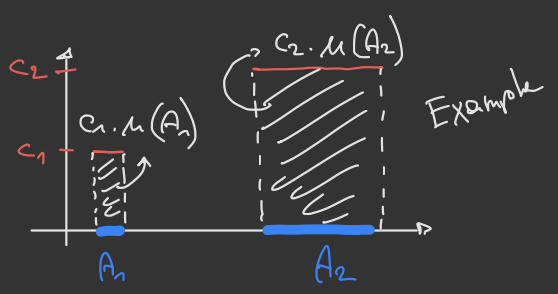
\includegraphics[width=0.5\linewidth]{figures/simple_function.png}
    \caption{Simple function 2}
    \label{fig:simplefunction2}
\end{figure}

We can then define the integral of $f$ as 
\begin{equation*}
    I(f) = \sum^n_{i=1} c_i \cdot \mu(A_i)
\end{equation*}

Problem: $\mu: F \to [0, \infty]$ and $c_i \in \mathbb{R} \implies$ we could get something like $10 \cdot \infty - 3 \cdot \infty$

Solution is

\begin{equation*}
    T^+ = \{f: S \to \mathbb{R}\, | f \text{ simple function and } f \geq 0 
\end{equation*}

For $f \in T^+$ we have a representation of $f$ as 
\begin{equation*}
    f(x) = \sum_{i=1}^n c_i \cdot \mathbb{1}_{A_i}(x) \text{ with } c_i \geq 0
\end{equation*}

and we can define the Lebesgue integral wrt. measure $\mu$ as 

\begin{equation*}
    I(f) = \sum_{i=1}^n c_i \cdot \mu(A_i)
\end{equation*}

Written in other notation: 
\begin{equation*}
    \int_S f \, d\mu \text{ or } \int_S f(x) \, d\mu(x)
\end{equation*}

This construction can be extended beyond simple function to all measureable functions $f: S\to \mathbb{R}$

One property: If $f$ and $g$ are lebesgue integrable, i.e., $\int f\, d\mu < \infty$ and $\int g\, d\mu < \infty$, and $f(x) \leq g(x)$, then 

\begin{equation*}
    \int f \, d\mu \leq \int g \, d\mu \, \ldots\text{ (Monotonicity property)}
\end{equation*}

We are now ready to state the definition of an expected value of a random variable. 

\begin{definition}
    Given a probability space $(S, \mathcal{F}, D)$ and a (quasi-integrable) random variable $X: S \to \mathbb{R}$, then we call $E[X]=\int_SX\,dD$ the expected value of $X$.
    Properties (without proof):
    \begin{enumerate}
        \item if $X\geq0$, then $E[X]\geq 9$
        \item E[X+Y]=E[X] + E[Y]
        \item $E[aX] = a E[X]$
        \item if $X\leq Y$ (almost everywhere, except for a set of measure 0), then $E[X] \leq E[Y|$ (given the exp. val. exists
    \end{enumerate}
\end{definition}

\subsubsection{Markov inequality}
Given a prob. space $(S,\mathcal{F}, D)$ and a non-negative random variable $X$, we have, for $a>0$:
\begin{equation*}
    \mathbb{P}[X\geq a]\leq \frac{E[X]}{a}
\end{equation*}

\begin{proof}
    Define $\mu:\, S \to \mathbb{R}$, $\varphi(x)=\begin{cases}
        a, \text{ if } X\geq a\\
        0,  \text{ if } X < a
    \end{cases}$
    Then, $0\leq \varphi(x)\leq X(x)$. Thus, by monotonicity we have:

    \begin{equation*}
    \int_S X\, dD = \int_S \varphi \,dD = a\cdot D\,(\{x\in S:\, X(x) \geq 0\})
    \end{equation*}

    since $a>0$, we can divide by $a$

    \begin{equation*}
        \frac{1}{a} \cdot \underset{E[X]}{\int_S X\,dD} \underset{\mathbb{P[X\geq a]}}{\geq D\,(\{x\in S:\, X(x)} \geq 0\})\implies \mathbb{P}[X \geq a]\leq \frac{E[X]}{a}
    \end{equation*}
\end{proof}

\newpage
\textcolor{red}{BREAK HERE}

Claim: 

\begin{align}
    \mathbb{E}[L_S(h)]&=L_{D,f}(h)\\
    Page \, 6
\end{align}

\textbf{Our first learning paradigm}\\
Empirical Risk Minimization (ERM) As a learner only has access to the training data ($S$), it is \textit{natural} to try to select $h$ (our hypothesis) such that the empirical risk (emp. error) is minimized. We call such a $h$ an empirical risk minimizer (an ERM hypothesis). 

\textbf{Example of a problematic case:}\\
\begin{figure}
    \centering
    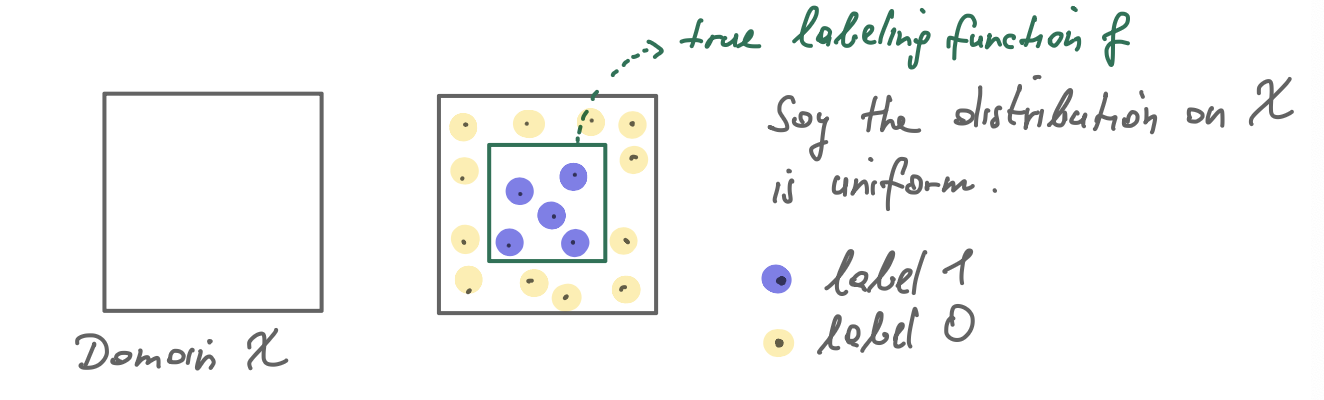
\includegraphics[width=1\linewidth]{figures/ExampleOfProblematicCase.png}
    \caption{Example of problemtic case}
    \label{fig:ProbCase}
\end{figure}

Also, assume that the area of the domain (square) is 2 and the area of the inner square is 1. 

Now, say we have an ERM algorithm that returns $h_S$, such that:

\begin{equation}
    h_s(x) = \begin{cases}
        y_i, \text{ if } \exists i \in \{1, \ldots, m\}: x_i =x \\
        0, \text{ else}
    \end{cases}
\end{equation}
Sort of a look up table


Obviously, $h_s$ is correct in all instances, if $S \to h_s$ is an empirical risk minimizer, meaning:
\begin{equation*}
    L_S(h_S) =0
\end{equation*}

But, on unseen instances from $D$ (which is uniform on $X$), $h_s$ is only correct 50\% of the time, leading to: 

\begin{equation*}
    L_{D,f}(h_s) = \frac{1}{2}
\end{equation*}

That's what we call \textit{overfitting}!


\textbf{Hypothesis class ($H$): (p.8)}\\
We restrict searching for $h$ to $H$, e.g. a class of functions from $X \to Y$ and we write 
\begin{equation}
    ERM_H (S) \in \underset{h \in H}{\arg \min} \,  L_S(H)
\end{equation}

\textbf{ERM over finite hypothesis class ($|H| < \infty$)}


Assumtion (realizability): $\exists h^* \in H$ with $L_{D,f}(h^*) =0$

Now, any ERM hypothesis $h_s$ will attain $0$ empirical error ($L_{D,f}(h_S)=0$) as $h_s$ competes against $h^*$ (which has $L_{D,f}(h^*) =0$ and obviously $L_S(h^*)=0$). 

We know that $L_{D,f}>\varepsilon,\, \varepsilon \in (0,1)$, can only happen if our learner selects a hypothesis $h_s$ with $L_S(h_S)=0$, \textbf{but} $L_{D,f}(h_S) > \varepsilon$.

We define a set of bad hypotheses: 
\begin{equation*}
    H_{\text{BAD}}=\{h \in H: L_{D,f} > \varepsilon\}
\end{equation*}

Also, we define: 
\begin{equation*}
    M=\{S|_X: \exists h \in H_{\text{BAD}}, L_S(h)=0\}
\end{equation*}

\textbf{Observation: p.9}



\textbf{p.11}\\
In words, the probability of the generalization error of an ERM hypothesis $h_s$ being larger of equal to $\varepsilon \in (0,1)$ is upper bounded by $|H|\cdot e^{-mc}$ (to be understood as the probability over a random draw of a dataset $S$ of size $m$, i.i.d. form $D$).

\textbf{Interlude (Markov inequality)}
We have a probability space $(S, \mathcal{F}, D)$ and a non-negative random variable $X$ ($X\geq 0$).




\begin{proof}{\textbf{Markov Inequality}}
    Claim: $\forall a >0$, we have: 
\begin{equation*}
    \mathbb{P}[X\geq a] \leq \frac{\mathbb{E}[X]}{a}
\end{equation*}
Define $\varphi:\, S\to \mathbb{R}$
\begin{equation*}
    \varphi(x)=\begin{cases}
        a, \, \text{if } x\geq a\\
        0, \, \text{else } (x < a)
    \end{cases}
\end{equation*}

\begin{figure}
    \centering
    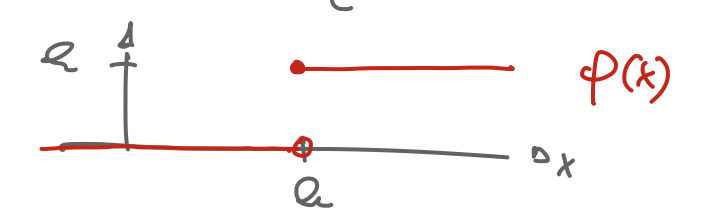
\includegraphics[width=0.5\linewidth]{figures/MarkovsIEQ.png}
    \label{fig:MarkIEQ}
\end{figure}

We have $0\leq \varphi(X(x)) \leq X(x)$ (for all $x\geq 0$)

\textbf{PAGE 12}

\end{proof}

\begin{corollary}
    Let $|H|<\infty$ and $\varepsilon, \delta \in (0,1)$. Further, let $m$ be an integer such that $m>\varepsilon^{-1}\log \, (|H| \delta^{-1})$. Then, for any labeling function $f: X \to \{0,1\}$ and any distribution $D$ (for which realizability holds), we have that with probability of at least $1-\delta$ over the choice of $S|_x$ of size $m$, every ERM hypothesis $h_S$ satisfies
    \begin{equation*}
        L_{D,f}(h_S) \leq \varepsilon
    \end{equation*}
    Interpretation: For sufficiently large m, $ERM_H$ returns a hypothesis $h_S$ that is Probably ($1-\delta$) approximately $\varepsilon$ Correct (PAC). 
\end{corollary}

\textbf{page 13}


\begin{definition}{PAC learnability}
    A hypothesis class $H$ is PAC learnable, if there exists a function $m_H:(0,1)^2 \to \mathbb{N}$ and a learning algorithm $A$ with the following properties. 1) For every $ \varepsilon, \delta \in (0,1)$ and 2) every distribution $D$ over the domain $X$ and 3) every labeling function $f:X\to \{0,1\}$, if 4) realizability holds (with respect to $H,\,D,\,f$), then running $A$ on $m \geq m_H (\varepsilon, \delta)$ i.i.d. instances form $D$ labeled by $f$), returns a hypothesis $h$, such that with probability at least $1-\delta$, it holds that
    \begin{equation*}
        L_{D,f}(h) \leq \varepsilon
    \end{equation*}
    
\end{definition}

\textbf{Terminology:}

$m_H: (0,1)^2 \to \mathbb{N}$ is called the sample complexity (function)

\textbf{page 14}

We now move to a more general setting, 

First, we will remove the realizability assumption, this means, there is no longer a $h^*\in H$ with $L_D,f(h^*)=0$. Now, the best possible thing that we can hope for is a guarantee relative to $\underset{h \in H}{\min} L_{D,f}(h)$ (before with realizability, this was 0!).

\begin{definition}[Höffding Inequality]
Let $X_1,\,\ldots \,,X_m $ i.i.d. random variables taking values in $[a_i, b_i] \text{ for } i \in \{1, \, \ldots \,, m \}$. Then, given that

\begin{equation*}
    S_m=\sum^m_{i=1} X_i
\end{equation*}

it holds that 

\begin{align*}
    \text{a)}& \quad \mathbb{P}[S_m -\mathbb{E}[S_m]>\varepsilon] \leq \exp \,\big (\frac{-2\varepsilon^2}{\sum_i{(b_i-a_i)^2}}\\
    \text{b)}& \quad \mathbb{P}[S_m -\mathbb{E}[S_m]<-\varepsilon] \leq \exp \,\big (\frac{-2\varepsilon^2}{\sum_i{(b_i-a_i)^2}}
\end{align*}

\textbf{Page 15}

and, upon combination (using union bound) 

\begin{equation*}
    \mathbb{P}[|S_m -\mathbb{E}[S_m]|>\varepsilon] \leq \exp \,\big (\frac{-2\varepsilon^2}{\sum_i{(b_i-a_i)^2}}
\end{equation*}

An alternative (quite useful) form is: 
\begin{equation*}
    \mathbb{P}[|\frac{1}{m} \sum_{i=1}^m X_i -\mu|>\varepsilon] \leq \exp \,\big (\frac{-2\varepsilon^2}{\sum_i{(b-a)^2}}
\end{equation*}
with $\mu = \mathbb{E}[X_i]$ and $\mathbb{P}[a\leq X_i \leq b]=1 \quad \forall i \in \{1, \ldots, m\}$.

As a consequence of this equation, we can already say the following: fix $\varepsilon > 0$; then, for a simple $h:X \to Y$, we have:

\begin{equation*}
    \underset{S|_x \sim D^m}{\mathbb{P}}[|L_s(h)-L_{D,f}(h)|>\varepsilon] \leq \exp \,\big (\frac{-2\varepsilon^2}{\sum_i{(b-a)^2}}    
\end{equation*}

since $a=0$ and $b=1$. Importantly, this only holds for a simple h!!!

\textbf{Page 16}

What we want is a bound that holds uniformly over all $h\in H$.

So, for $|H| < \infty$ (finite classes), we can get (by the union bound):

\begin{align*}
    \underset{S|_x \sim D^m}{\mathbb{P}}[\forall h \in H: |L_s(h)-L_{D,f}(h)|>\varepsilon] &\leq \sum_{h \in H} 2e^{-2\varepsilon^2m}\\   
    &\leq |H|2e^{-2\varepsilon^2m}
\end{align*}

Remark: we did not need realizability for that! But, we pay the price of $\varepsilon^2$ vs. $\varepsilon$.

Secondly, we get rid of the true leabeling function $f:X \to Y$ (which labeled our training instances $x_i$) by letting $D$ be adistribution over $X \times Y$, e.g. over domain and label space ($Y$).

\textbf{Page 17}

Let $Z:X \times Y$. We need to adjust our definitions of empirical error and generalization error. 

\begin{align*}
    L_D(h) &= \underset{(x,y) \sim D}{\mathbb{P}}[h(x) \neq y] = D\, \big ( \{(x,y) \in X \times Y: h(x) \neq y\} \big )\\
    L_S(h) &= \frac{1}{m} \cdot \bigl| \big \{i \in \{1, \ldots, m\}: h(x_i) \neq y_i\big \} \bigr |
\end{align*}

\end{definition}

\begin{definition}[Agnostic PAC learnability]
    
\end{definition}

\end{document}

